\documentclass[10pt]{article}

\usepackage[margin=0.75in]{geometry}
\usepackage{amsmath,amsthm,amssymb,bm}
\usepackage{xcolor}
\usepackage{cancel}
\usepackage{graphicx}
\usepackage{changepage}
\usepackage{circuitikz}
\usepackage{pgfplots}
\usepackage{minted}
\usepackage{physics}
\usepackage{hyperref}
\usepackage{siunitx}
\usepackage{fontspec}
\usepackage{relsize}
\usepackage{subfig}
\usepackage{todonotes}
\usepackage{multicol, multirow, booktabs}
\usepackage[breakable]{tcolorbox}
\usepackage[inline]{enumitem}

\usepackage{ifthen}
\usepackage{tikz,pgfplots}
\usepackage{tikz-3dplot}
\usepackage{auto-pst-pdf}
\usepackage{pstricks}
\usepackage{pst-magneticfield}

\theoremstyle{definition}
\newtheorem{problem}{Problem}
\newtheorem{soln}{Solution}

\pgfplotsset{compat=newest}
\usetikzlibrary{lindenmayersystems}
\usetikzlibrary{arrows}
\usetikzlibrary{calc}
\usetikzlibrary{positioning, fit}
\usetikzlibrary{3d, perspective}


\definecolor{incolor}{HTML}{303F9F}
\definecolor{outcolor}{HTML}{D84315}
\definecolor{cellborder}{HTML}{CFCFCF}
\definecolor{cellbackground}{HTML}{F7F7F7}
\newcommand{\ui}{\hat{i}}
\newcommand{\uj}{\hat{j}}
\newcommand{\uk}{\hat{k}}
\newcommand{\ux}{\hat{\mathbf{x}}}
\newcommand{\uy}{\hat{\mathbf{y}}}
\newcommand{\uz}{\hat{\mathbf{z}}}
\newcommand{\uv}[1]{\hat{\bv{{#1}}}}
\newcommand{\pr}[1]{{#1^\prime}}
\newcommand{\pd}[2][]{{\frac{\partial^{#1}}{\partial {{#2}^{#1}}}}}
\newcommand{\dif}[2][]{{\frac{d^{#1}}{d{{#2}^{#1}}}}}
\pgfdeclarelayer{background}  
\pgfsetlayers{background,main}
\AtBeginDocument{\RenewCommandCopy\qty\SI}

\makeatletter
\newcommand{\boxspacing}{\kern\kvtcb@left@rule\kern\kvtcb@boxsep}
\makeatother
\newcommand{\prompt}[4]{
    \ttfamily\llap{{\color{#2}[#3]:\hspace{3pt}#4}}\vspace{-\baselineskip}
}

\newcommand{\thevenin}[2]{
  \begin{center}
    \begin{circuitikz} \draw
      (0,0) -- (2,0) to[battery1, l_=$V_{Th}\eq#1$] (2,2) 
      to[resistor, l_=$R_{Th}\eq#2$] (0,2)
      ;
      \draw [o-] (-.07,2.079);
      \draw [o-] (-.07,0.079);
    \end{circuitikz}
  \end{center}
}

\newcommand{\norton}[2]{
  \begin{center}
    \begin{circuitikz} \draw
      (0,0) -- (3,0) to[american current source, l_=$I_{N}\eq#1$] (3,2) -- (0,2) (2,0)
      to[resistor, l=$R_{N}\eq#2$] (2,2)
      ;
      \draw [o-] (-.07,2.079);
      \draw [o-] (-.07,0.079);
    \end{circuitikz}
  \end{center}
}

\DeclareMathOperator{\Div}{div}
\DeclareMathOperator{\Curl}{curl}
\DeclareMathOperator{\sgn}{sgn}

\DeclareSIUnit\foot{ft}

\newcommand{\highlight}[1]{\colorbox{yellow}{$\displaystyle #1$}}

\newcommand{\ti}[1]{\widetilde{#1}}

\newfontface{\Kaufmann}{Kaufmann}
\DeclareTextFontCommand{\kf}{\Kaufmann}
\newcommand{\scriptr}{\fontsize{12pt}{12pt}\kf{r}}

\newfontface{\KaufmannB}{Kaufmann Bold}
\DeclareTextFontCommand{\kfb}{\KaufmannB}
\newcommand{\bscriptr}{\fontsize{12pt}{12pt}\kfb{r}}
\newcommand{\justif}[2]{&{#1}&\text{#2}}
\newcommand{\bv}[1]{\bm{\mathrm{#1}}}


\title{Physics 3200Y: Lab III Discussion}
\author{Jeremy Favro (0805980) \\ Trent University, Peterborough, ON, Canada}
\date{\today}

\begin{document}
\maketitle

% PROBLEM 1
\begin{problem}
Record your design parameters and adjust them as appropriate for optimization. Qualitatively
test the accuracy of the Lorentz force law by operating at varying factors.
\end{problem}
\begin{soln}
  Obviously as I am submitting this afterthe fact I can't record ay design parameters. In lab we tested the Lorentz force law by
  varying field strength and direction by moving the magnet and by attempting different coil geometries to see if greater torque could be achieved
  with a rectangle.
\end{soln}
\newpage
% PROBLEM 2
\begin{problem}
Redraw Fig. 2 with labels and a circuit. Test each variable's magnitude and direction.
\end{problem}
\begin{soln}
  I obviously can't verify this but the varables were tested qualitatively in lab.
  \begin{center}
    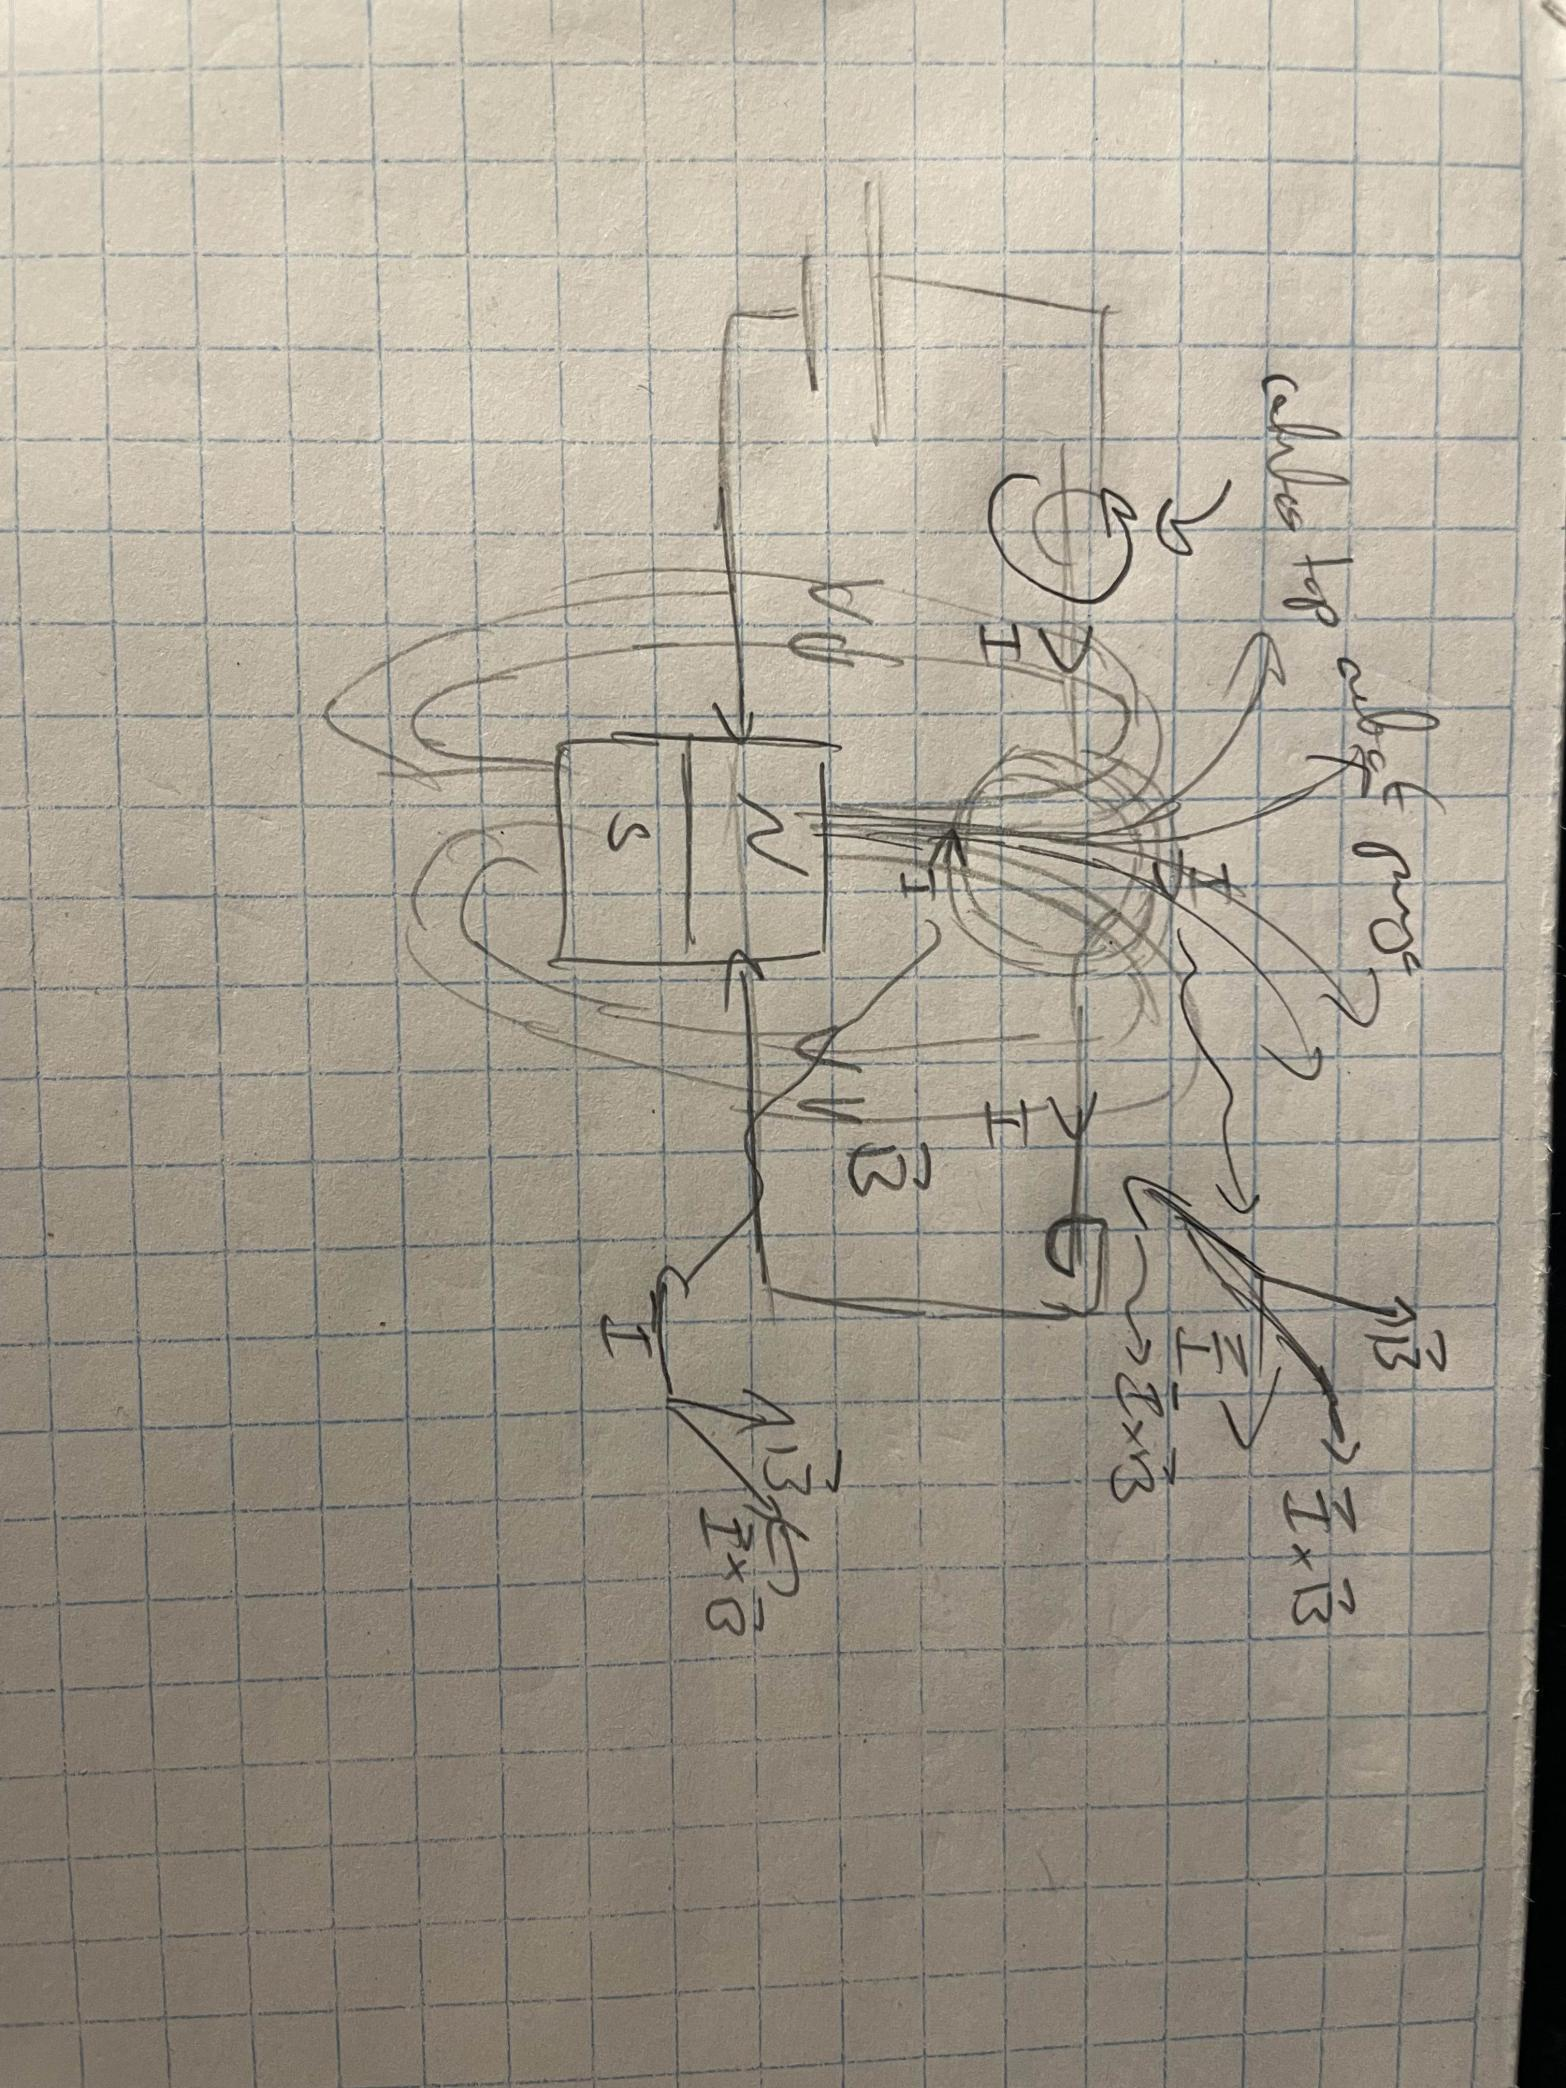
\includegraphics[scale=0.3, angle=90]{fig.jpg}
  \end{center}
\end{soln}
\newpage

% PROBLEM 3
\begin{problem}
For the DC motor:
\begin{enumerate}[label=(\alph*)]
  \item What if the coil terminals were taped non-collinearly, i.e., not on the same side of the shaft?
  \item What if you were to tape the wires $\pm\qty{90}{\degree}$ on the shaft?
  \item What if the coil shape design were rectangular?
  \item Which variable is, in practice, the easiest to adjust to increase the motor's torque by 100x?
\end{enumerate}
For both the loudspeaker and the motor:
\begin{enumerate}[label=(\alph*)]
  \item Do the coils' movement/rotation obey the Lorentz force?
  \item What would be affected if you changed only the AWG size? \# of turns?
  \item Have you considered the non-uniformity and tri-dimensionality of the B-field?
  \item Did the coil heat up significantly? How will you redesign to account for coil heating?
  \item Enumerate ways on how to optimize and increase the efficiency of your devices. Have you encountered limitations?
\end{enumerate}
\end{problem}
\begin{soln}
  For the DC motor:
  \begin{enumerate}[label=(\alph*)]
    \item The motor would fail to function as there must be a completed circuit at some point for current to flow and a torque to be induced.
    \item This would make the coil jump laterally (perpendicular to the axis) when the circuit is completed.
    \item I think in the case we had in lab a rectangular shape would be (and was) worse than a circular shape. We tested a very large rectangle and found that the
          torque produced was insufficient, however a smaller rectangle worked but was also worse than the circular coils. I believe this is due to the fact
          that the magnet we were given was smaller in diameter than any of our coils, the field lines wouldn't form right-angles with the edges of a rectangle on the long sides
          which eliminates the advantage of using a rectangle. I want to say that this also helps the circular coil as the way I imagine the field lines would have them intersecting
          may more points than just the top and bottom of the circular coils at right-angles, however I cannot be sure of this as I could not see the field lines from the
          magnet given in lab.
    \item Since the torque felt bythe motor grows linearly with everything but the diameter I am tempted to say multiplying the diameter by 10. This
          would be inconvenient though so probably just increasing the number of turns by winding more regularly and densly. This also has the benefit of not singificantly
          increasing the moment of inertia of the coil.
  \end{enumerate}
  For both the loudspeaker and the motor:
  \begin{enumerate}[label=(\alph*)]
    \item Yeah.
    \item Decreasing AWG might allow for more current flow and hence more torque as resistance decreases with AWG. This would also probably cause more heating.
          Increasing the number of turns would create greater torque by exposing more current to the field at a given time. These are both the same in the case of the speaker though I think
          most of the optimization there would mroe be in cone design.
    \item Yes, see my answer to part (c) in the previous set of questions. In the case of the speaker this is not so much of an issue as the magnets were pre-assembled 
    to create a radial field where the coil sits.
    \item The smaller coils (with greater AWG) produced less heat than the larger ones which had a smaller AWG. To cheaply reduce heating I think we could reduce current
          and increase the number of coils, however more in-depth thought on this is wanted as increasing winding density could also lead to trapping of excess heat.
          In the case of the speaker I think the only real optimizations possible would be a cone material that is a good thermal conductor and denser coils so that head from the inner turns
          can more eaisly radiate through the coil outwards.
    \item The biggest thing I wanted to try was to mount the coil axle on bearings and mount the brushes seperately. There was significant
          vibration when the coil was spinning as when contact was made the coil experienced forces in directions other than the strictly torque inducing one.
          Fixing the axis would reduce the jumping and allow for smoother rotation. Cleaner, more regular winding might also help to ensure that when contact is made
          the angle between the field and the current is optimal in all coils. External brushes rather than the setup in lab where the coil rode on the brushes
          would allow for a more consistent point ofcontact and hence greater optimization to do with the relative angle of the coil and contactors.
          For the speaker I think perpendiculary stabilizing (perpendicular to the cone opening) the speaker cone would help so that lateral movement is lessend and 
          there is hence less friction between the cone and the magnets. Re-working the wire connections would also probably help, in the configuration used in lab they were
          definitely restricting the movement of the cone.
  \end{enumerate}
\end{soln}
\end{document}